\documentclass{report}
\usepackage{geometry}
 \geometry{
 a4paper,
 total={170mm,257mm},
 left=20mm,
 top=20mm,
 }

% Damit die Verwendung der deutschen Sprache nicht ganz so umst\"andlich wird,
% sollte man die folgenden Pakete einbinden: 
\usepackage[latin1]{inputenc}% erm\"oglich die direkte Eingabe der Umlaute 
\usepackage[T1]{fontenc} % das Trennen der Umlaute
\usepackage{ngerman} % hiermit werden deutsche Bezeichnungen genutzt und 
                     % die W\"orter werden anhand der neue Rechtschreibung 
             % automatisch getrennt. 
\usepackage{graphicx}
\usepackage{comment}
\graphicspath{ {./test_preamp/} }
\usepackage{subcaption}
\newcommand{\sectionbreak}{\clearpage}
\usepackage[section]{placeins}
\title{Documentation Preamps testing}


\date{04.05.2021}
% Hinweis: \title{um was auch immer es geht}, \author{wer es auch immer 
% geschrieben hat} und  \date{wann auch immer das war} k\"onnen vor 
% oder nach dem  Kommando \begin{document} stehen 
% Aber der \maketitle Befehl mu\ss{} nach dem \begin{document} Kommando stehen! 
\begin{document}

\maketitle




\section{Setup 0}
For this testing the setup of the FOPRA was used. The preamps were tested on the big box with the five large crystals inside. The small box (with 8 small crystals) was used as reference to check if there are RCBus interferences. As the five crystals of the large box are connected to one single Sub-D connector, the signal processing from the APDs to the output of the MPRB could only be tested for 5 channels on the Preamp card 0. For all other channels the test was done solely using the pulser. As pulser signal a square signal shape (low end: 0mV, high end: 10mV, 50\% duty) with frequency of 250 Hz.


\newpage

\section{Test Results} \label{documentclasses}
All following plots are uncalibrated lim\textunderscore energy plots. The pulser peak can be identified as the most right peak in the plots. 

\subsection{Preamp 1, Max. Range 3pC/30pC}
To repair: All channels in both cards noisy.
\begin{figure}[!htb]
  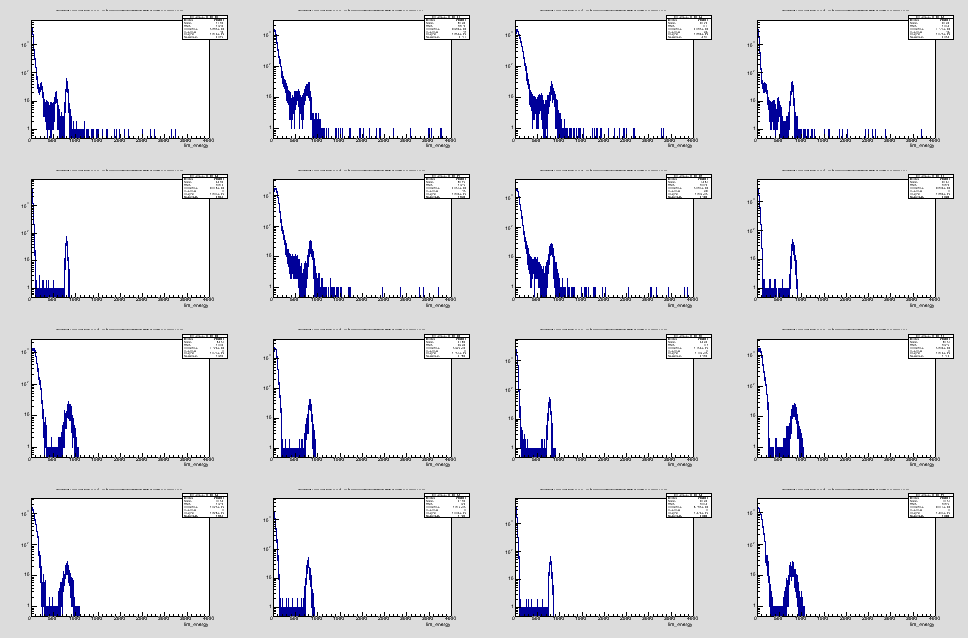
\includegraphics[width=\linewidth]{preamp1_lim_energy_card0_all.png}
  \caption{Preamp 1, card 0, all channels, Na22 source  with pulser. All channels noisy.}
\end{figure}

\begin{figure}[!htb]
  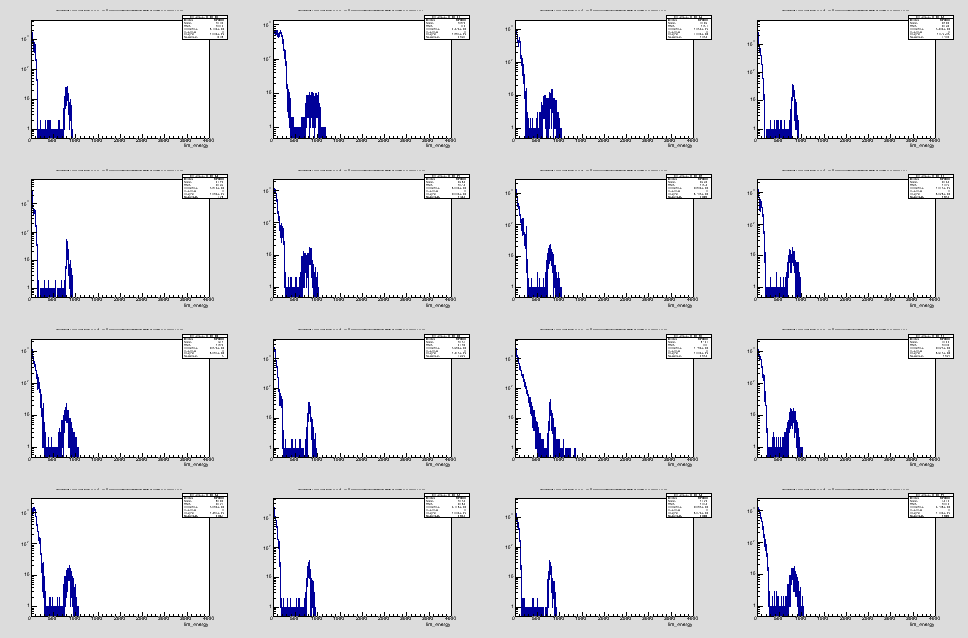
\includegraphics[width=\linewidth]{preamp1_lim_energy_card1_all.png}
  \caption{Preamp 1, card 1, all channels, no crystal, only pulser. All channels noisy.}
\end{figure}
\newpage
\clearpage

\subsection{Preamp 5, Max. Range 3pC/30pC}
To repair: card 0, missing channels 2 and 16 (FEBEXCh.5 and 9).
\begin{figure}[!htb]
  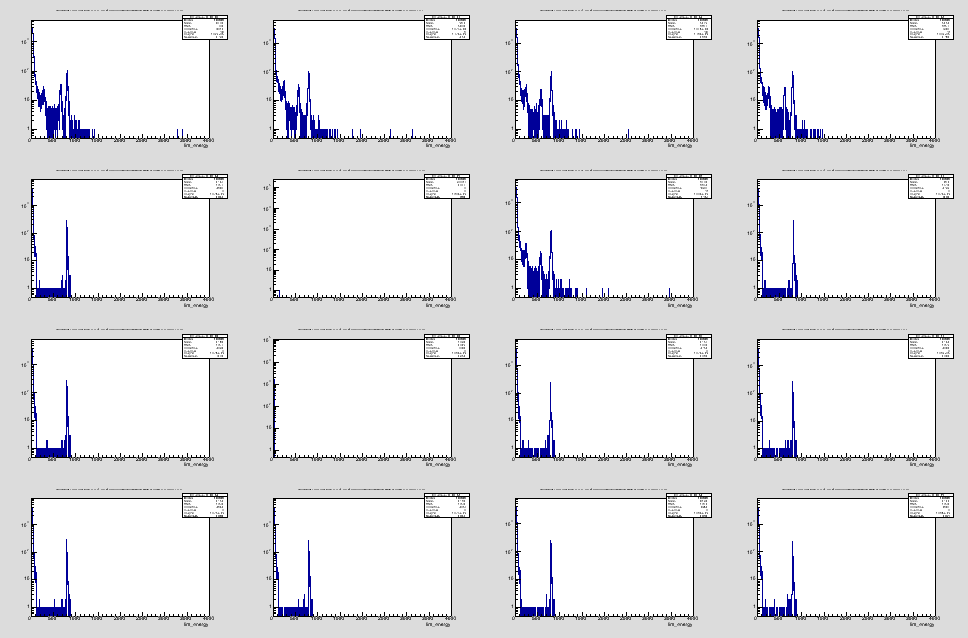
\includegraphics[width=\linewidth]{preamp5_lim_energy_card0_all.png}
  \caption{Preamp 5, card 0, all channels, Na22 source  with pulser. Missing channels 2 and 16 (FEBEXCh.5 and 9).}
\end{figure}
\newpage
\clearpage

\subsection{Preamp 6 (Dual Range), Max. Range 3pC/30pC}
To repair: card 0 channels 8,9,10,11,12,15 (FEBEXCh. 7,8,10,13,14,15) are noisy. card1 channels 7,8,9,10,11,12,13,15 (FEBEXCh. 0,7,8,10,12,13,14,15) are noisy.
\begin{figure}[!htb]
  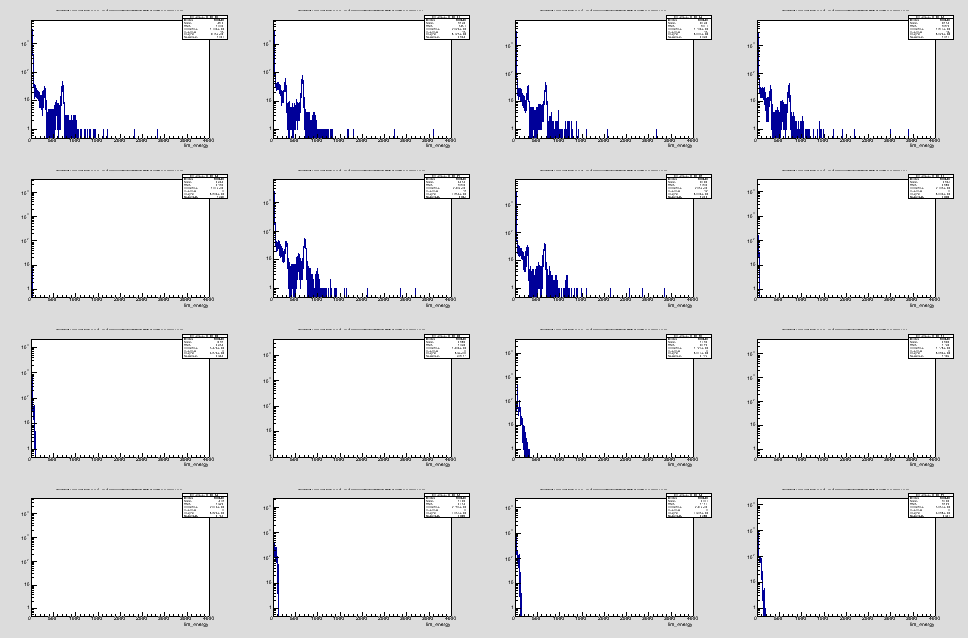
\includegraphics[width=\linewidth]{/dr_latest_test/preamp6_lim_energy_card0_all_no_pulser.png}
  \caption{Preamp 6, card 0, all channels, Na22 source  no pulser. Channels 8,9,10,11,12,15 (FEBEXCh. 7,8,10,13,14,15) are noisy }
\end{figure}

\begin{figure}[!htb]
  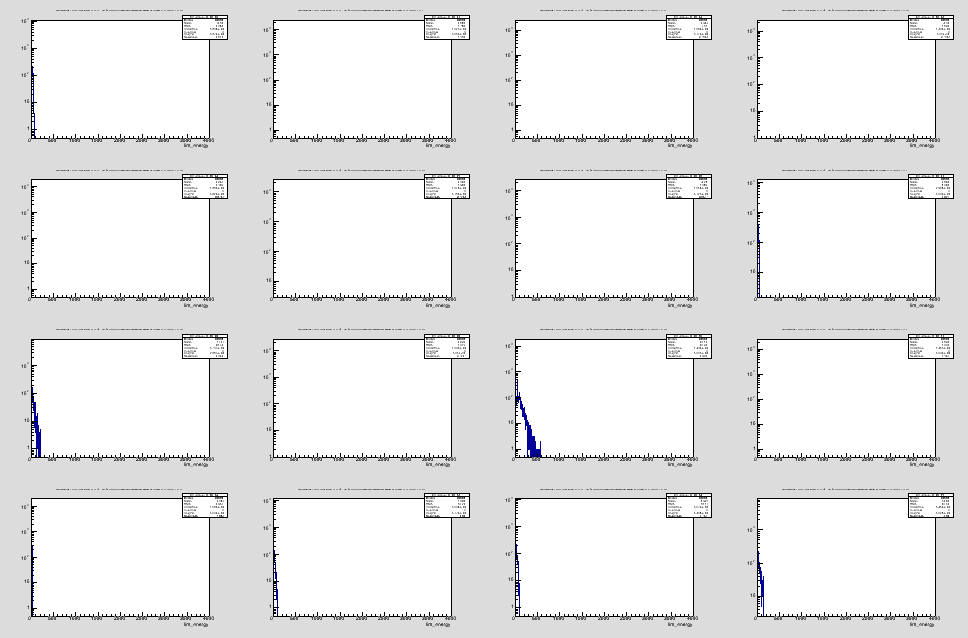
\includegraphics[width=\linewidth]{dr_latest_test/preamp6_lim_energy_card1_all_no_pulser.png}
  \caption{Preamp 6, card 1, all channels, Na22 source  no pulser. Channels 7,8,9,10,11,12,13,15 (FEBEXCh. 0,7,8,10,12,13,14,15) are noisy.}
\end{figure}
\newpage
\clearpage

\subsection{Preamp 7 (Dual Range), Max. Range 3pC/30pC}
To repair: card 1 channels 7,8,9,10,11,12,15 (FEBEXCh. 0,7,8,10,13,14,15) are noisy.
\begin{figure}[!htb]
  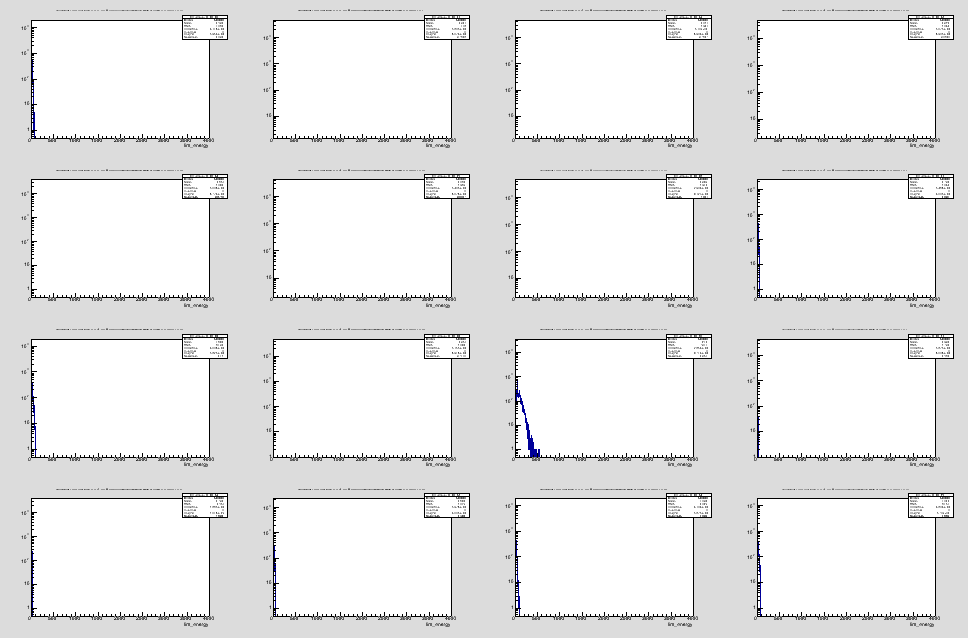
\includegraphics[width=\linewidth]{dr_latest_test/preamp7_lim_energy_card1_all_no_pulser.png}
  \caption{Preamp 7, card 1, all channels, Na22 source  no pulser. Channels 7,8,9,10,11,12,15 (FEBEXCh. 0,7,8,10,13,14,15) are noisy.}
\end{figure}

\newpage
\clearpage

\subsection{Preamp 8 (Dual Range), Max. Range 3pC/30pC}
To repair: card 0 all channels noisy. Card1 all channels are noisy.
\begin{figure}[!htb]
  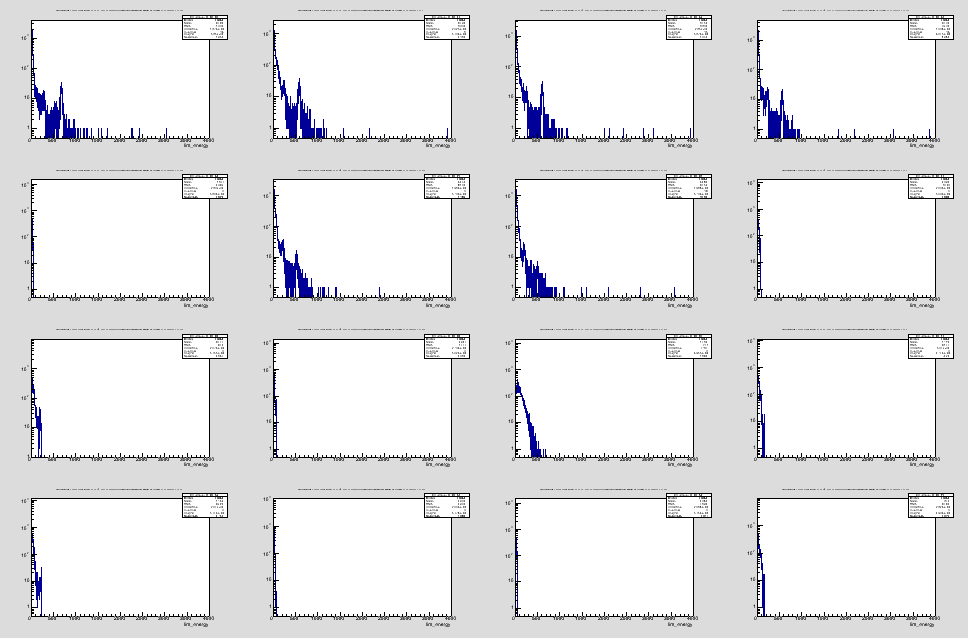
\includegraphics[width=\linewidth]{dr_latest_test/preamp8_lim_energy_card0_all_no_pulser.png}
  \caption{Preamp 8, card 0, all channels, Na22 source  no pulser. All channels are noisy.}
\end{figure}

\begin{figure}[!htb]
  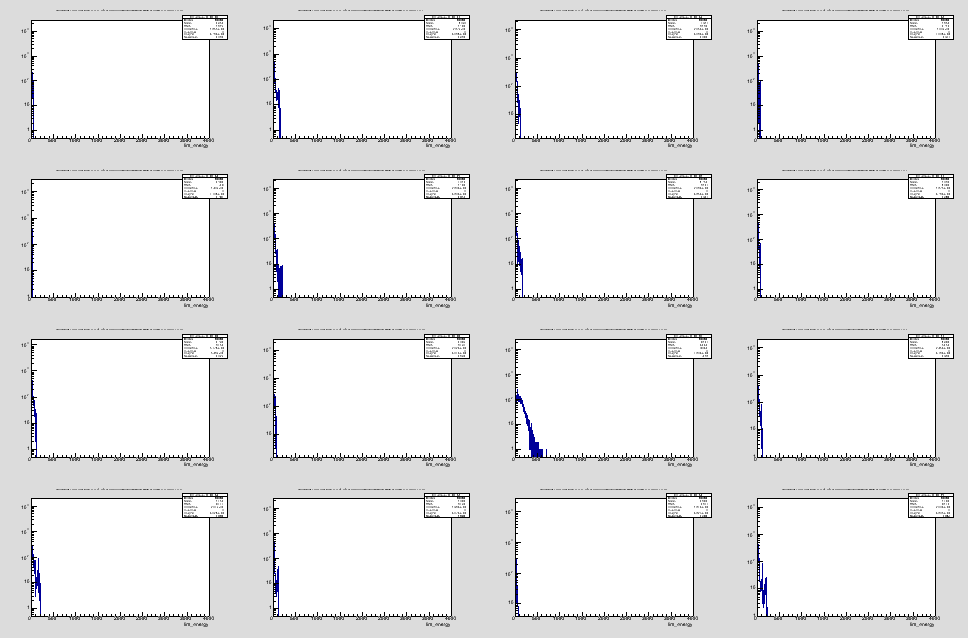
\includegraphics[width=\linewidth]{dr_latest_test/preamp8_lim_energy_card1_all_no_pulser.png}
  \caption{Preamp 8, card 1, all channels, Na22 source  no pulser. All channels are noisy.}
\end{figure}
\newpage
\clearpage

\subsection{Preamp 9 (Dual Range), Max. Range 3pC/30pC}
To repair: card1, channels 5,6,8,9,10,11,12,15 (FEBEXCh. 1,2,7,8,10,13,14,15) noisy. This can only be seen when lowering the \dq gamma\textunderscore discr\textunderscore threshold\dq{} from 500 to 100. More details in the RC-Bus Test.
\newpage
\clearpage

\subsection{Preamp 10, Max. Range 1pC/10pC}
To repair: card0 channels 8,9,10,11,12,15 (FEBEXCh. 7,8,10,13,14,15) are noisy.
\begin{figure}[!htb]
  \includegraphics[width=\linewidth]{small_box_card0_all_nopulser.png}
  \caption{Preamp 10, card 0, all channels, Na22 source  no pulser. Channels 8,9,10,11,12,15 (FEBEXCh. 7,8,10,13,14,15) are noisy.}
\end{figure}

\newpage
\clearpage


\section{RC-Bus Test - Setup}
For this test the preamps were detached from the detectors, they were operated free-standing. The gamma\textunderscore discr\textunderscore threshold was lowered to 100  (instead of 500, as before) to be able to identify more accurately noise caused from remote control requests. For the remote control requests a small python script using the pySerial API was employed. For the test all available preamp parameters were read individually, in a row and other combinations. All preamps were affected by noise when requesting the \dq Temp\textunderscore slope \dq{} or \dq Temp\textunderscore offset \dq{} parameter, or when requesting both of them in a loop. When putting \dq Temp\textunderscore slope \dq{} or \dq Temp\textunderscore offset \dq{} parameter in front of a requesting loop (e.g.: ask Temp\textunderscore slope, Voltage 8, Sum current) the noise effect was also observed. Setting the \dq Temp\textunderscore slope\dq{} or \dq Temp\textunderscore offset\dq{} parameter read request not in front of a requesting loop (e.g: ask Voltage 8,Temp\textunderscore slope,Sum current), no noise was observed.\newline
The following plots show the noise effect in the preamp channels  when requesting \dq Temp\textunderscore offset\dq{} with a frequency of 5 Hz. In all preamps the channels 1,2,3 (FEBEXCh. 6,5,4) are affected by the remote control request in decreasing magnitude.\newline
The plots are all in the 1pC and 3pC range as no signal is detected beyond this region.\newline

\subsection{Preamp 1, Max. Range 3pC/30pC}
\begin{figure}[!htb]
  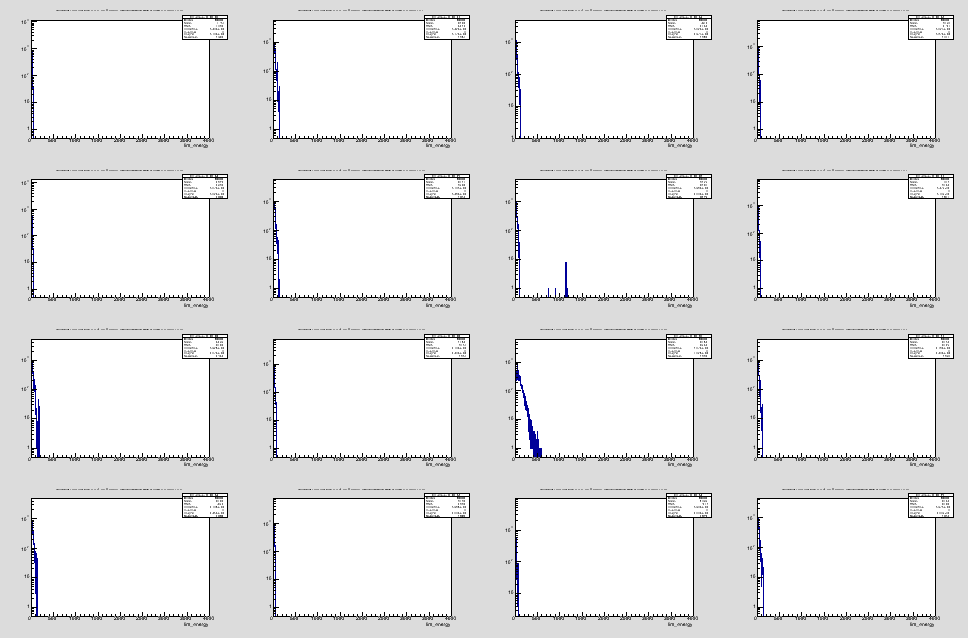
\includegraphics[width=\linewidth]{rc_bus_test/preamp1_card0_gamma_all.png}
  \caption{Preamp 1, card 0, all channels, preamp detached. Overall noise, nevertheless noise from parameter read request in channel 1 (FEBEXCh. 6) can clearly be identified.}
\end{figure}
\begin{figure}[!htb]
  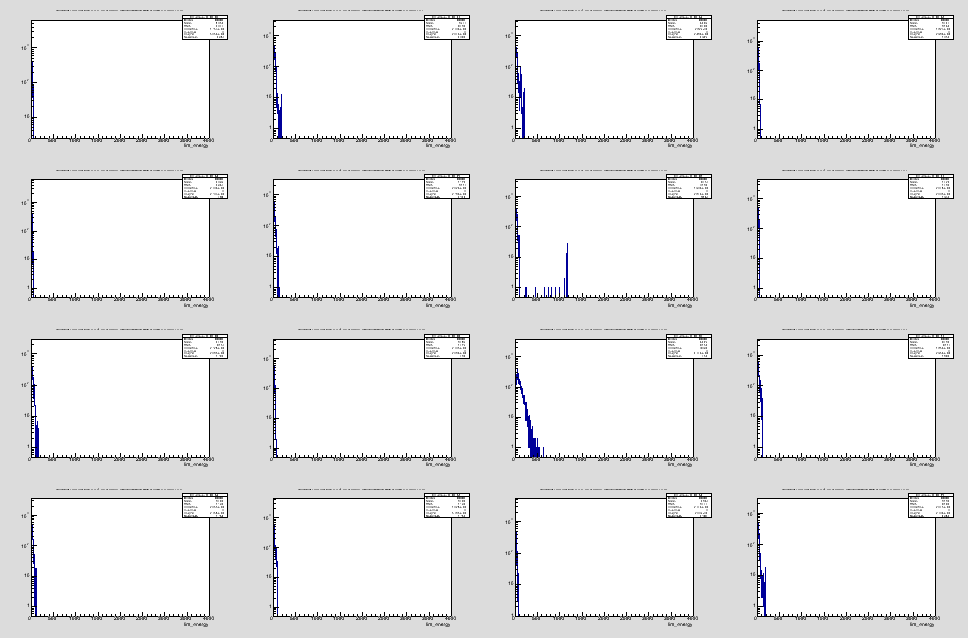
\includegraphics[width=\linewidth]{rc_bus_test/preamp1_card1_gamma_all.png}
  \caption{Preamp 1, card 1, all channels, preamp detached. Overall noise, nevertheless noise from parameter read request in channel 1 (FEBEXCh. 6) can clearly be identified.}
\end{figure}

\newpage
\clearpage


\subsection{Preamp 5, Max. Range 3pC/30pC}
\begin{figure}[!htb]
  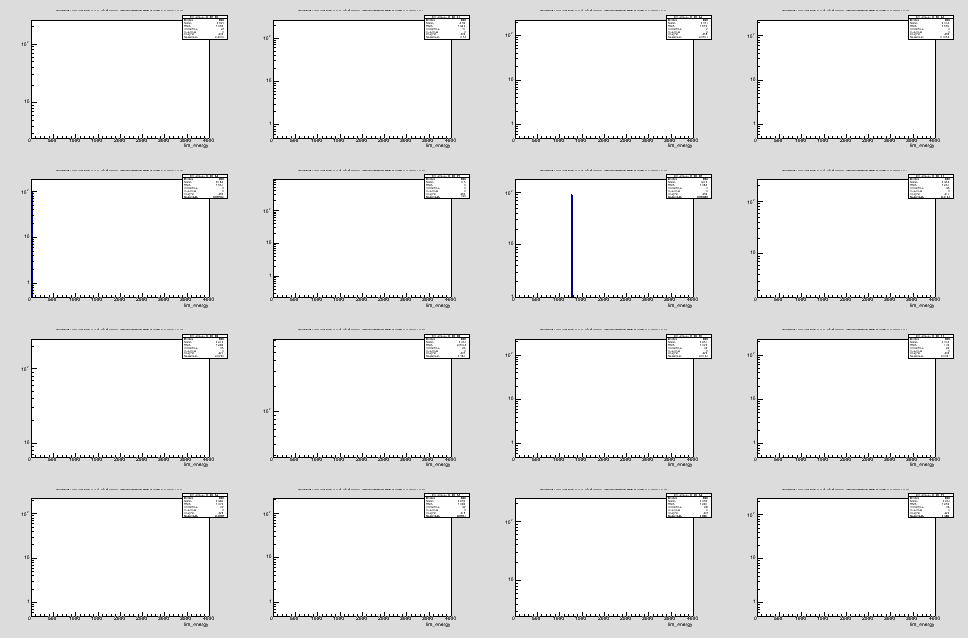
\includegraphics[width=\linewidth]{rc_bus_test/preamp5_card0_gamma_all.png}
  \caption{Preamp 5, card 0, all channels, preamp detached. Noise from parameter read request in channel 1,3 (FEBEXCh. 6,4).}
\end{figure}
\begin{figure}[!htb]
  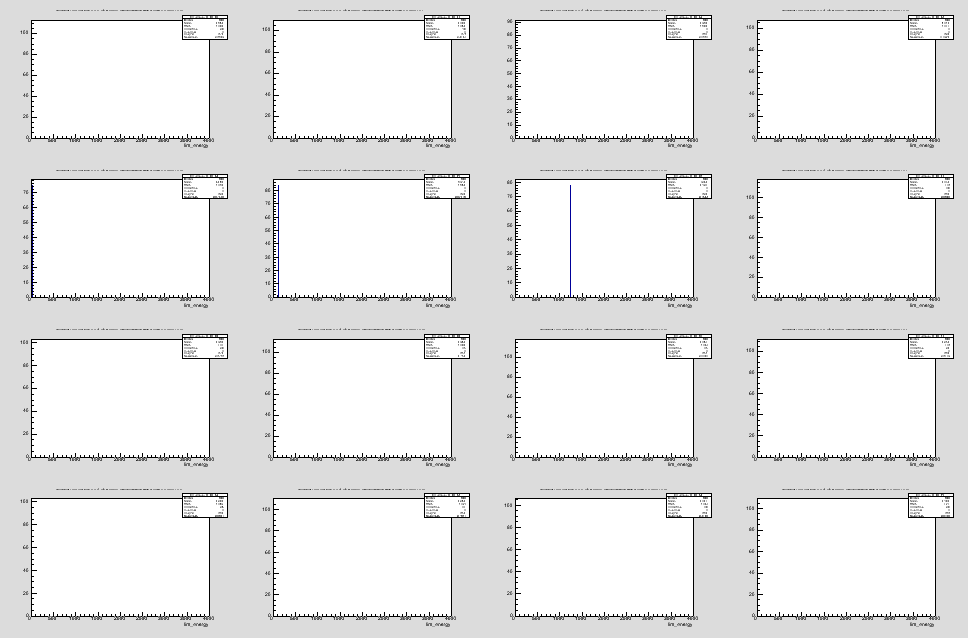
\includegraphics[width=\linewidth]{rc_bus_test/preamp5_card1_gamma_all.png}
  \caption{Preamp 5, card 1, all channels, preamp detached. Noise from parameter read request in channel 1,2,3 (FEBEXCh. 6,5,4).}
\end{figure}

\newpage
\clearpage


\subsection{Preamp 6 (Dual Range), Max. Range 3pC/30pC}
\begin{figure}[!htb]
  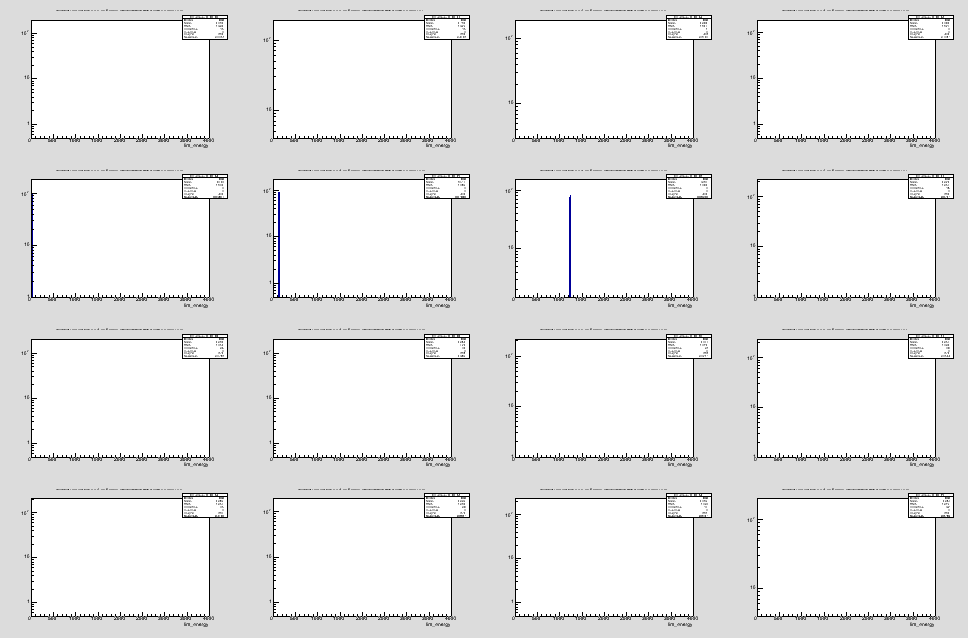
\includegraphics[width=\linewidth]{rc_bus_test/preamp6_card0_gamma_all.png}
  \caption{Preamp 6, card 0, all channels, preamp detached. Noise from parameter read request in channel 1,2,3 (FEBEXCh. 6,5,4,).}
\end{figure}
\begin{figure}[!htb]
  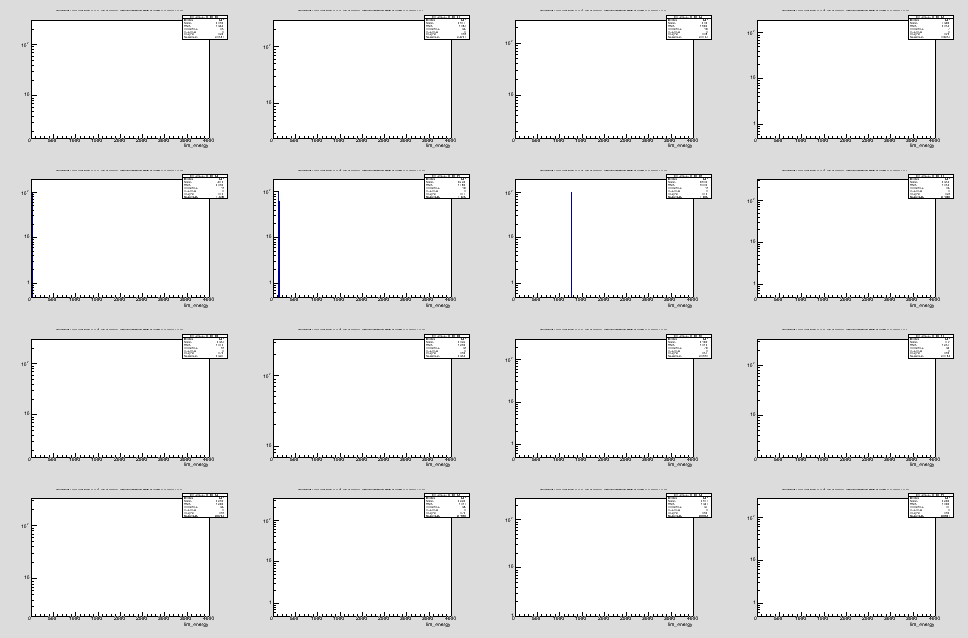
\includegraphics[width=\linewidth]{rc_bus_test/preamp6_card1_gamma_all.png}
  \caption{Preamp 6, card 1, all channels, preamp detached. Noise from parameter read request in channel 1,2,3 (FEBEXCh. 6,5,4,).}
\end{figure}

\newpage
\clearpage

\subsection{Preamp 7 (Dual Range), Max. Range 3pC/30pC}
\begin{figure}[!htb]
  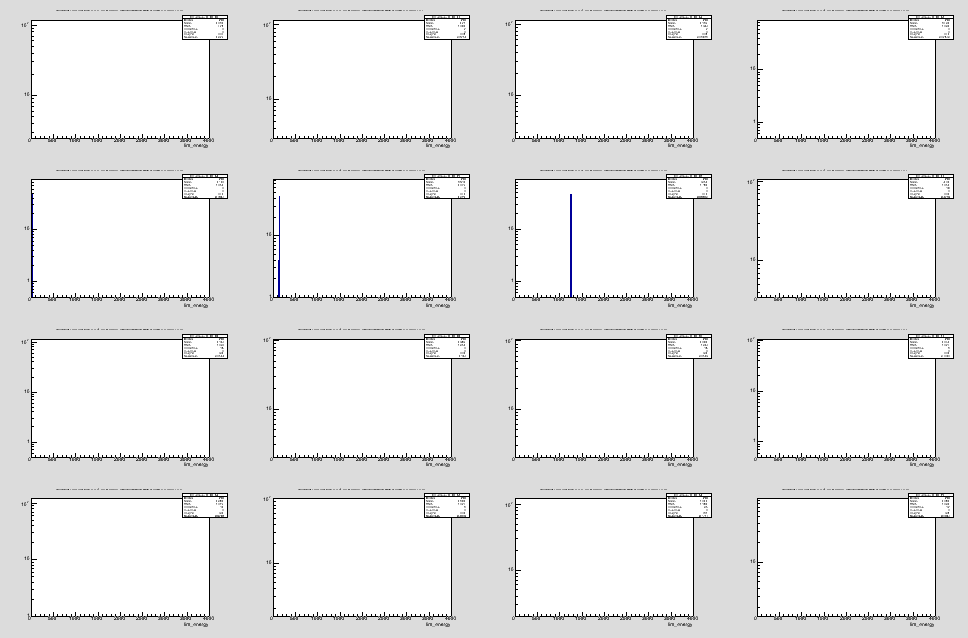
\includegraphics[width=\linewidth]{rc_bus_test/preamp7_card0_gamma_all.png}
  \caption{Preamp 7, card 0, all channels, preamp detached. Noise from parameter read request in channel 1,2,3 (FEBEXCh. 6,5,4,).}
\end{figure}
\begin{figure}[!htb]
  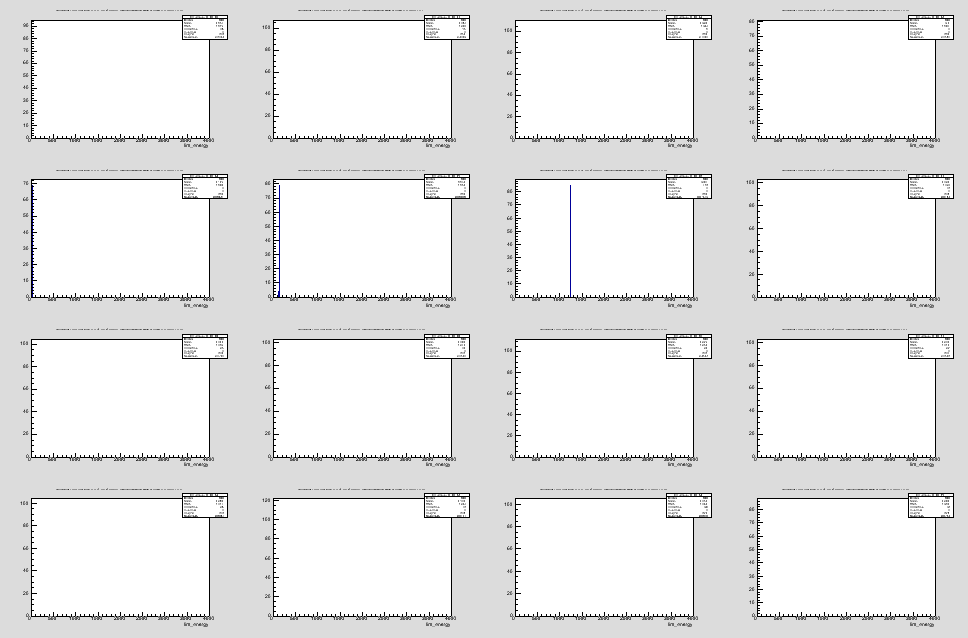
\includegraphics[width=\linewidth]{rc_bus_test/preamp7_card1_gamma_all.png}
  \caption{Preamp 7, card 1, all channels, preamp detached. Noise from parameter read request in channel 1,2,3 (FEBEXCh. 6,5,4,).}
\end{figure}

\newpage
\clearpage

\subsection{Preamp 8 (Dual Range), Max. Range 3pC/30pC}
\begin{figure}[!htb]
  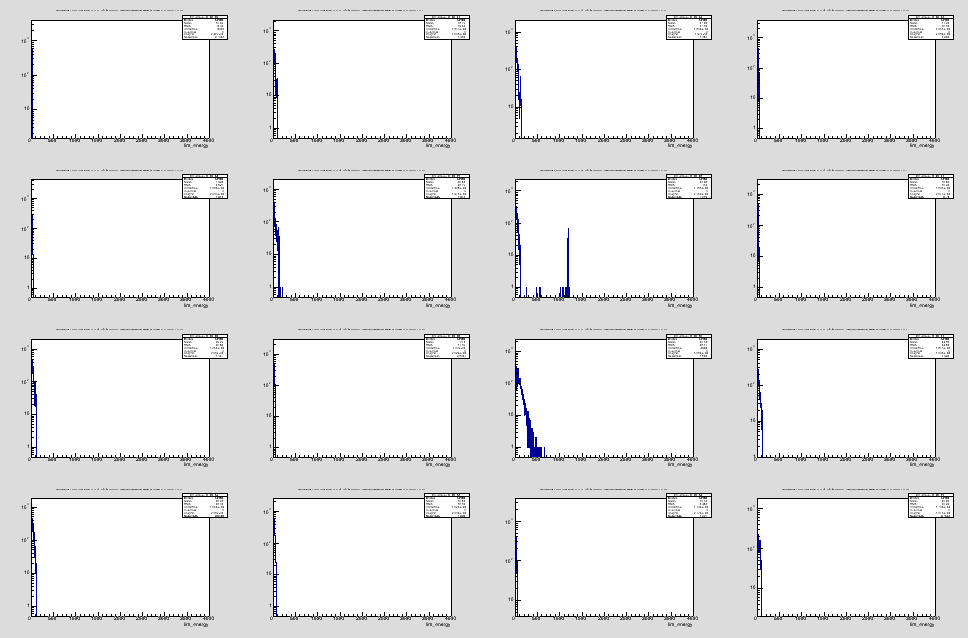
\includegraphics[width=\linewidth]{rc_bus_test/preamp8_card0_gamma_all.png}
  \caption{Preamp 8, card 0, all channels, preamp detached. Overall noise, nevertheless noise from parameter read request in channel 1 (FEBEXCh. 6) can clearly be identified.}
\end{figure}
\begin{figure}[!htb]
  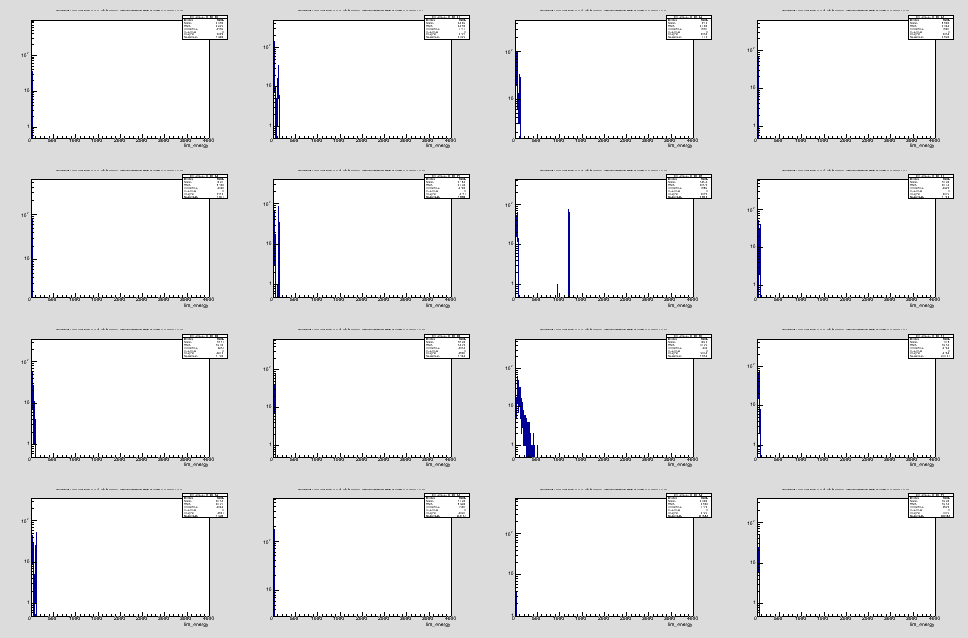
\includegraphics[width=\linewidth]{rc_bus_test/preamp8_card1_gamma_all.png}
  \caption{Preamp 8, card 1, all channels, preamp detached. Overall noise, nevertheless noise from parameter read request in channel 1,2 (FEBEXCh. 6,5) can clearly be identified.}
\end{figure}

\newpage
\clearpage

\subsection{Preamp 9 (Dual Range), Max. Range 3pC/30pC}
\begin{figure}[!htb]
  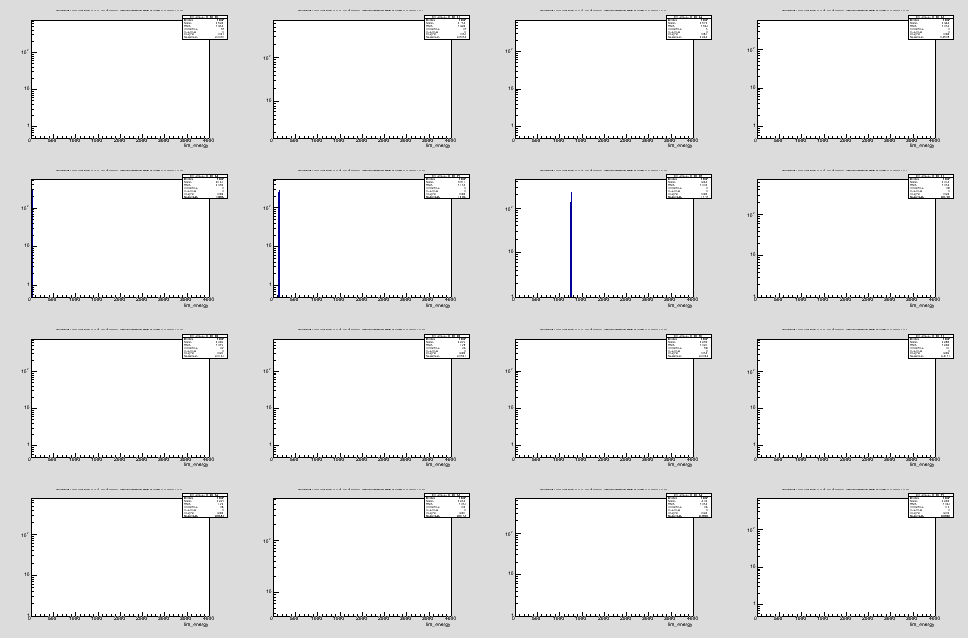
\includegraphics[width=\linewidth]{rc_bus_test/preamp9_card0_gamma_all.png}
  \caption{Preamp 9, card 0, all channels, preamp detached. Noise from parameter read request in channel 1,2,3 (FEBEXCh. 6,5,4).}
\end{figure}
\begin{figure}[!htb]
  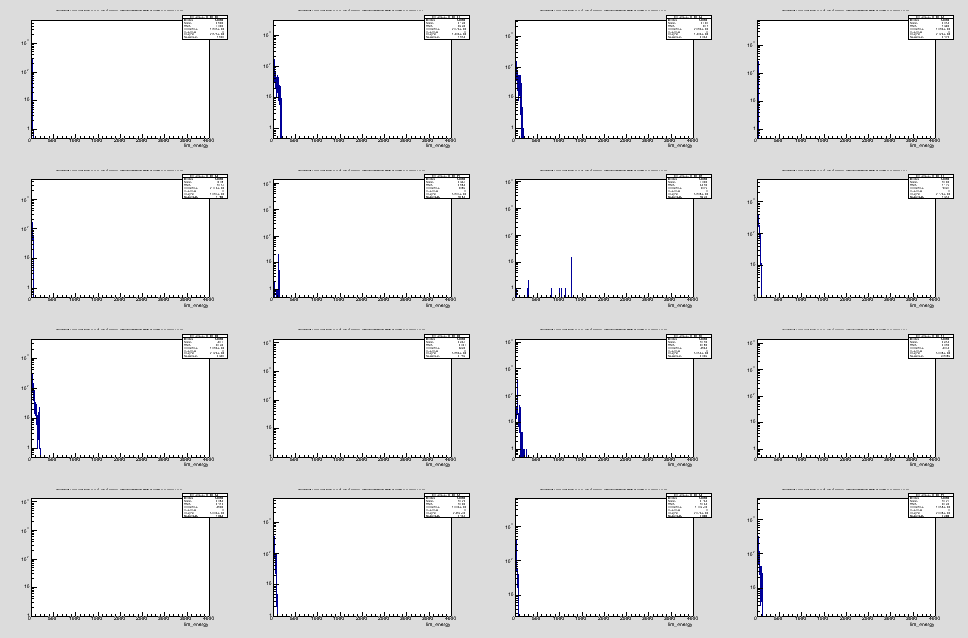
\includegraphics[width=\linewidth]{rc_bus_test/preamp9_card1_gamma_all.png}
  \caption{Preamp 9, card 1, all channels, preamp detached. Channels 5,6,8,9,10,11,12,15 (FEBEXCh. 1,2,7,8,10,13,14,15), nevertheless noise from parameter read request in channel 1,2,3 (FEBEXCh. 6,5,4).}
\end{figure}

\newpage
\clearpage

\subsection{Preamp 10, Max. Range 1pC/10pC}
\begin{figure}[!htb]
  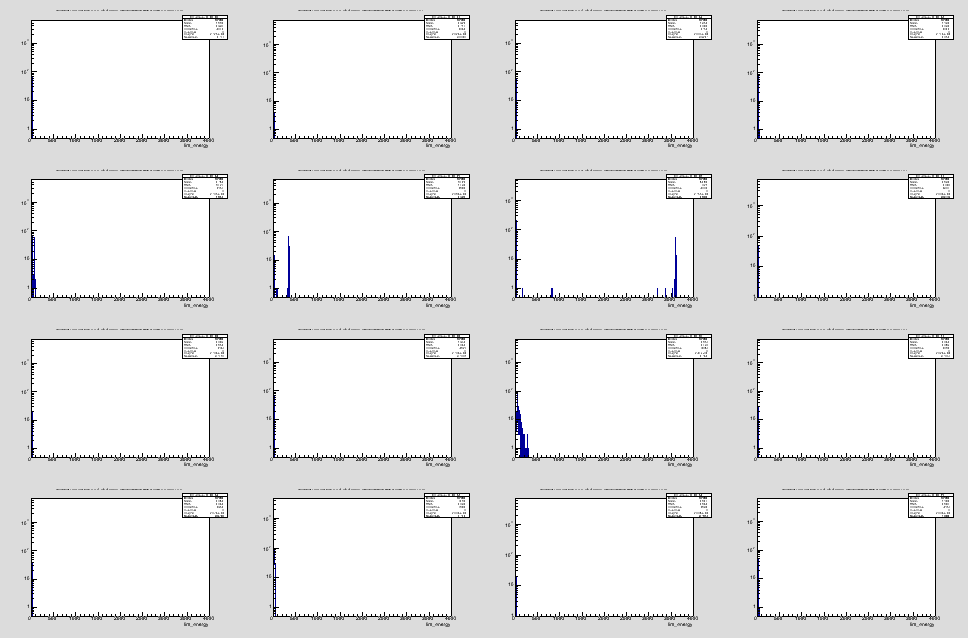
\includegraphics[width=\linewidth]{rc_bus_test/preamp10_card0_gamma_all.png}
  \caption{Preamp 10, card 0, all channels, preamp detached. Channel 15 (FEBEXCh.10)  noisy, nevertheless noise from parameter read request in channel 1,2,3 (FEBEXCh. 6,5,4) can clearly be identified.}
\end{figure}
\begin{figure}[!htb]
  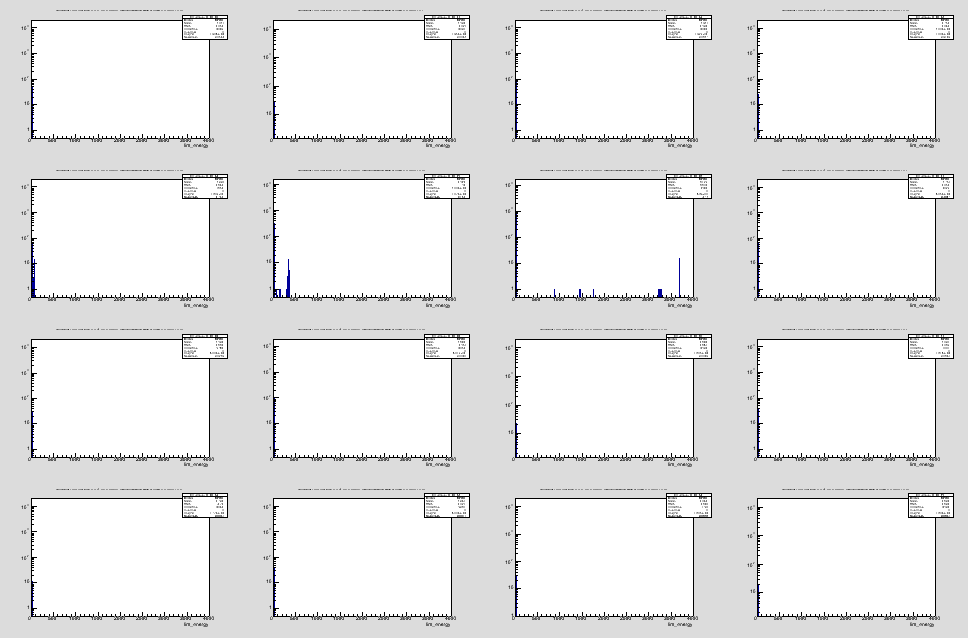
\includegraphics[width=\linewidth]{rc_bus_test/preamp10_card1_gamma_all.png}
  \caption{Preamp 10, card 1, all channels, preamp detached. Noise from parameter read request in channel 1,2,3 (FEBEXCh. 6,5,4).}
\end{figure}

\newpage
\clearpage







\section{Summary - repair demand}
Preamp 1, seems to be noisy in both cards (0,1), bad resolultion.\newline
Preamp 5, card 0: here we have missing channels 2 and 16.\newline
Preamp 6, card 0: 8,9,10,11,12,15 channels are noisy. card 1: 7,8,9,10,11,12,13,15 channels are noisy.\newline
Preamp 7, card 1: 7,8,9,10,11,12,15 channels are noisy\newline
Preamp 8, card0: all channels are noisy. card1: all channels noisy\newline
Preamp 9, card1: 5,6,8,9,10,11,12,15 are noisy.\newline
Preamp10,card 0: 8,9,10,11,12,15 channels noisy.\newline
\newpage


\section{Backup}
With the same two setup the FOPRA Preamp(Max. Range 1pC/10pC) was tested. Even though it has a noisy/broken channel 15 (FEBEXCh. 10) on card1 it cannot be brought to repair, as we need it for the FOPRA. (The good thing is that the broken channel does not affect the FOPRA experiment, as for the FOPRA only card0 is used).

\begin{figure}[!htb]
  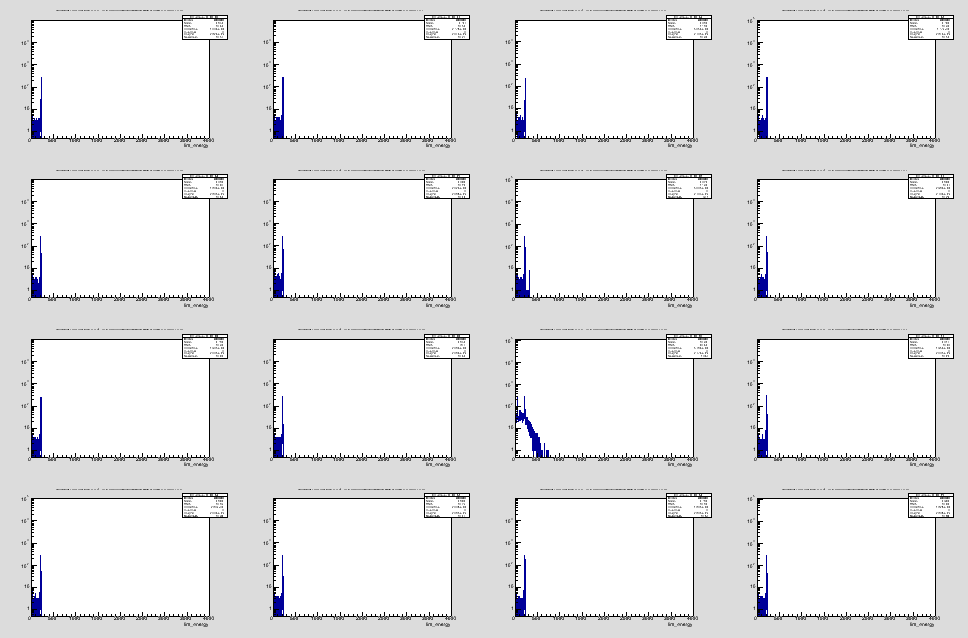
\includegraphics[width=\linewidth]{fopra_preamp_lim_energy_card1_all.png}
  \caption{Setup 0 with pulser. FOPRA Preamp, card 1, all channels, no crystal, only pulser. Channel 15 (FEBEXCh. 10) noisy/broken.}
\end{figure}
\begin{figure}[!htb]
  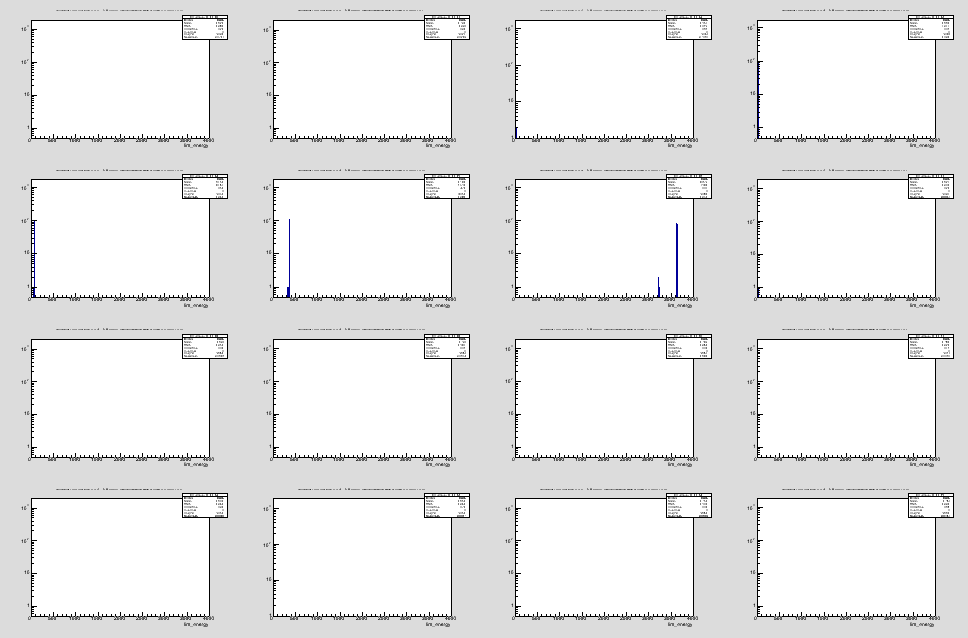
\includegraphics[width=\linewidth]{rc_bus_test/preampfopra_card0_gamma_all.png}
  \caption{RC-Bus-Setup. Preamp FOPRA, card 0, all channels, preamp detached. Noise from parameter read request in channel 1,2,3,4 (FEBEXCh. 6,5,4,3).}
\end{figure}
\begin{figure}[!htb]
  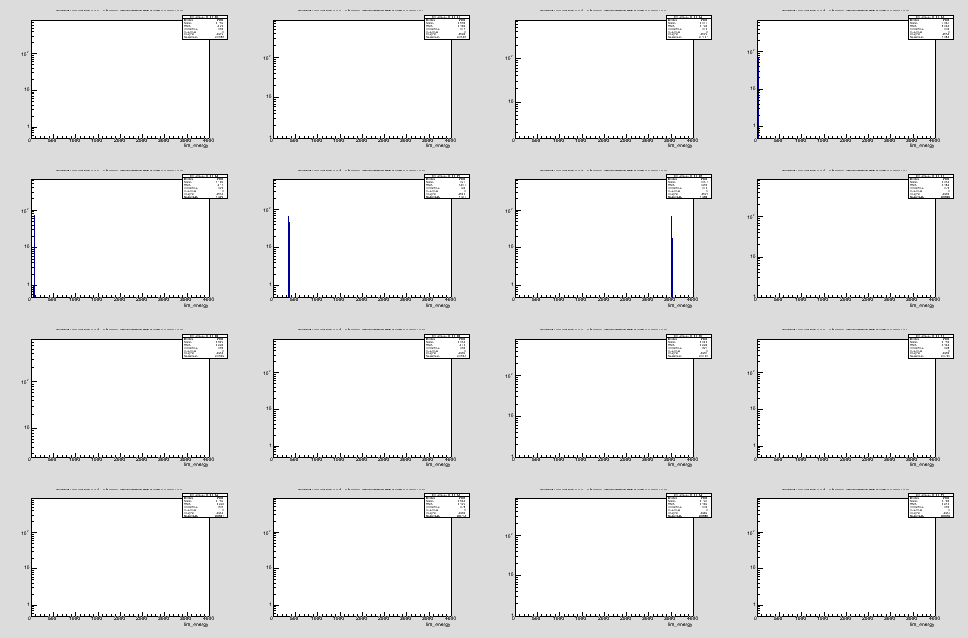
\includegraphics[width=\linewidth]{rc_bus_test/preampfopra_card1_gamma_all.png}
  \caption{RC-Bus-Setup. Preamp FOPRA, card 1, all channels, preamp detached. Noise from parameter read request in channel 1,2,3,4 (FEBEXCh. 6,5,4,3).}
\end{figure}


\end{document}


